% Adapted from code found in:
%https://tex.stackexchange.com/questions/171169/how-to-draw-a-simple-cone-with-height-and-radius-with-tikz?fbclid=IwAR0533AG6I6Owsw3P5Tl7wXwZ_Vais7BJGly11duBR4emmQPwMM2gQeiGYU

\documentclass[tikz,border=2mm]{standalone} 
\usetikzlibrary{positioning, calc}

\begin{document}

    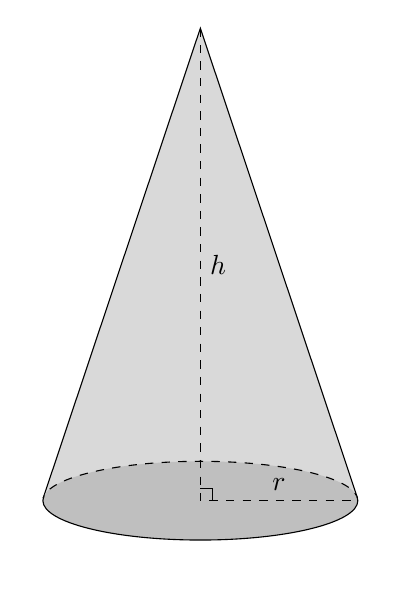
\begin{tikzpicture}

        \newcommand{\radiusx}{2}
        \newcommand{\radiusy}{.5}
        \newcommand{\height}{6}

        \newcommand{\pointX}{{\radiusx*sqrt(1-(\radiusy/\height)*(\radiusy/\height))}}
        \newcommand{\pointY}{{\radiusy*(\radiusy/\height)}}

        \coordinate (a) at (-\pointX,\pointY);
        \coordinate (b) at (\pointX,\pointY);

        \draw[fill=gray!30] (a)--(0,\height)--(b)--cycle;
        \fill[gray!50] circle (\radiusx{} and \radiusy);

        \begin{scope}
            \clip ([xshift=-2mm]a) rectangle ($(b)+(1mm,-2*\radiusy)$);
            \draw circle (\radiusx{} and \radiusy);
        \end{scope}

        \begin{scope}
            \clip ([xshift=-2mm]a) rectangle ($(b)+(1mm,2*\radiusy)$);
            \draw[dashed] circle (\radiusx{} and \radiusy);
        \end{scope}

        \draw[dashed] (0,\height)|-(\radiusx,0) node[right, pos=.25]{$h$} node[above,pos=.75]{$r$};

        \draw (0,.15)-|(.15,0);
    \end{tikzpicture}
\end{document}